% !TEX encoding = IsoLatin

\documentclass[11pt,a4paper]{article}
\usepackage[latin1]{inputenc}
\usepackage[spanish]{babel}
\usepackage[T1]{fontenc}
\usepackage{amsmath,amssymb}
\usepackage{wrapfig}
\usepackage{bm}
\usepackage{graphicx,color}
\usepackage{fancyhdr}
\usepackage{hyperref}
\usepackage{enumitem}
\usepackage[top=0.6in,left=0.8in,body={170mm,270mm}]{geometry}
\usepackage{blindtext}

\begin{document}
\thispagestyle{empty}


%\noindent





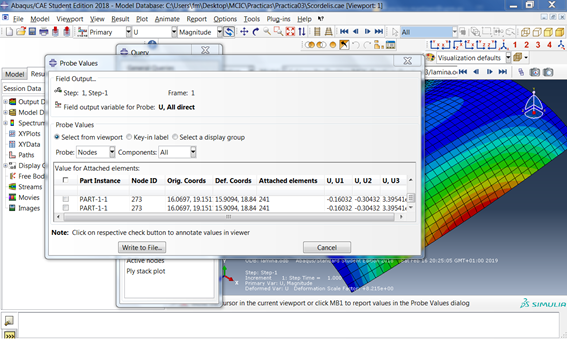
\includegraphics{Fig-1_Despla_Vertical.png}

\centering{Figura 1: Desplazamiento Vertical}
\vspace{3cm}


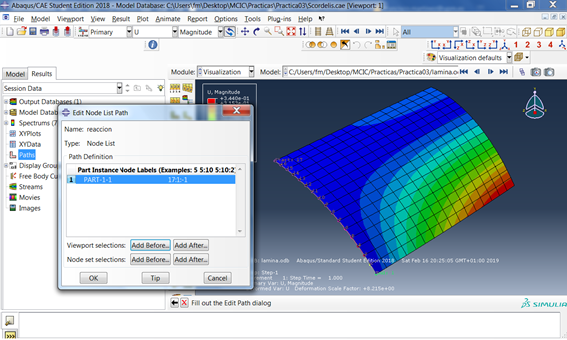
\includegraphics{Fig-2_Reacc_Vertical.png}

\centering{Figura 2: Path Reacci�n Vertical}
\vspace{3cm}


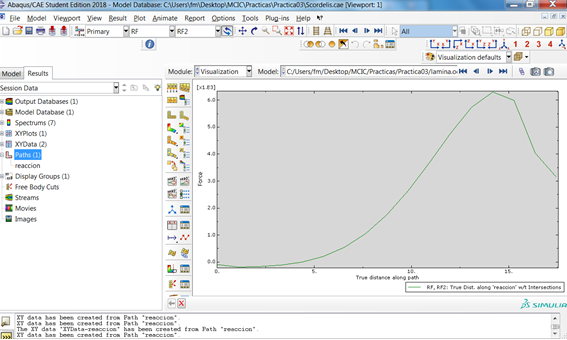
\includegraphics{Fig-3_Reacc_Vertical_longitud.png}

\centering{Figura 3:Reacci�n vertical por unidad de longitud}

\vspace{3cm}

Integral de la reacci�n por unidad de longitud:
\vspace{1cm}

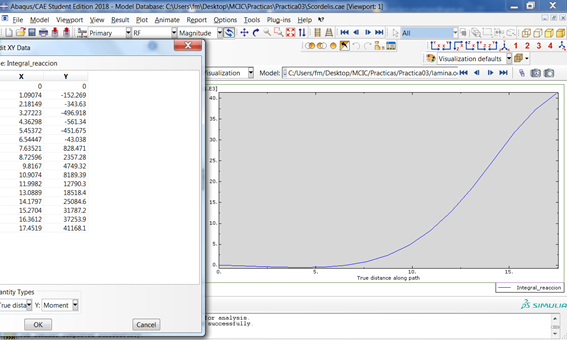
\includegraphics{Fig-4_Integral_Reacc_Vertical}

\centering{Figura 4: Integral reacci�n vertical}
\vspace{3cm}

Si hacemos los c�lculos de la reacci�n total:
\vspace{1cm}
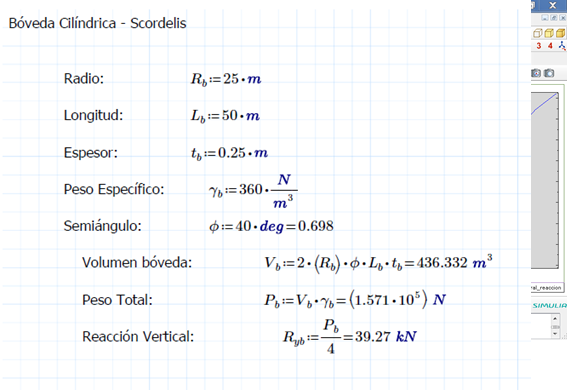
\includegraphics{Fig-5_Analitico_Reacc_Vertical}

\centering{Figura 5: C�lculo anal�tico reacci�n}
\vspace{3cm}


Que difiere ligeramente (5%).
La raz�n, es que la opci�n {\it pathi} no es la forma m�s exacta de sumar reacciones ya que hay una interpolaci�n de por medio. La forma correcta ser�a sumar las reacciones individuales de cada uno de los nodos como se aprecia a continuaci�n:

\vspace{1cm}
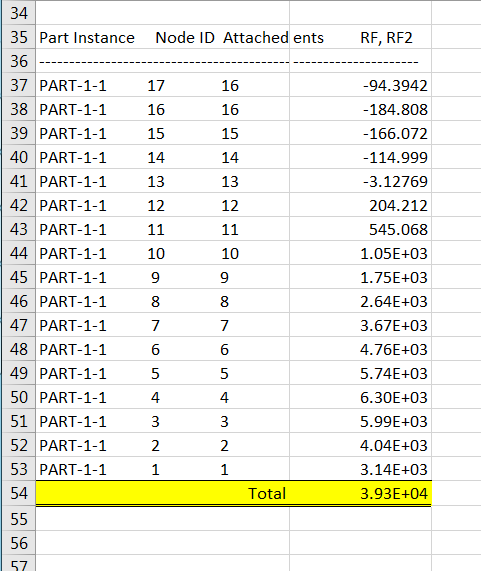
\includegraphics{Fig-6_Suma_reacciones.png}

\centering{Figura 6: Suma reacciones nodales}
\vspace{3cm}




Una forma de hacerlo sin tener que {\it sumarlas manualmente} es establecer una
restricci�n de todos los nodos  del borde de inter�s a un �nico nodo mediante
un {\it MPC} o un {\it kinematic coupling} y recuperar la reacci�n en dicho nodo.
Para ello al borde anterior se acopla una restricci�n cinem�tica a un �nico nodo que puede ser real o ficticio y al que se fija la condici�n de contorno fija. De este modo la reacci�n obtenida es la correspondiente a la resultante total de ese borde. En este caso el nodo maestro es uno de los v�rtices:

\vspace{1cm}

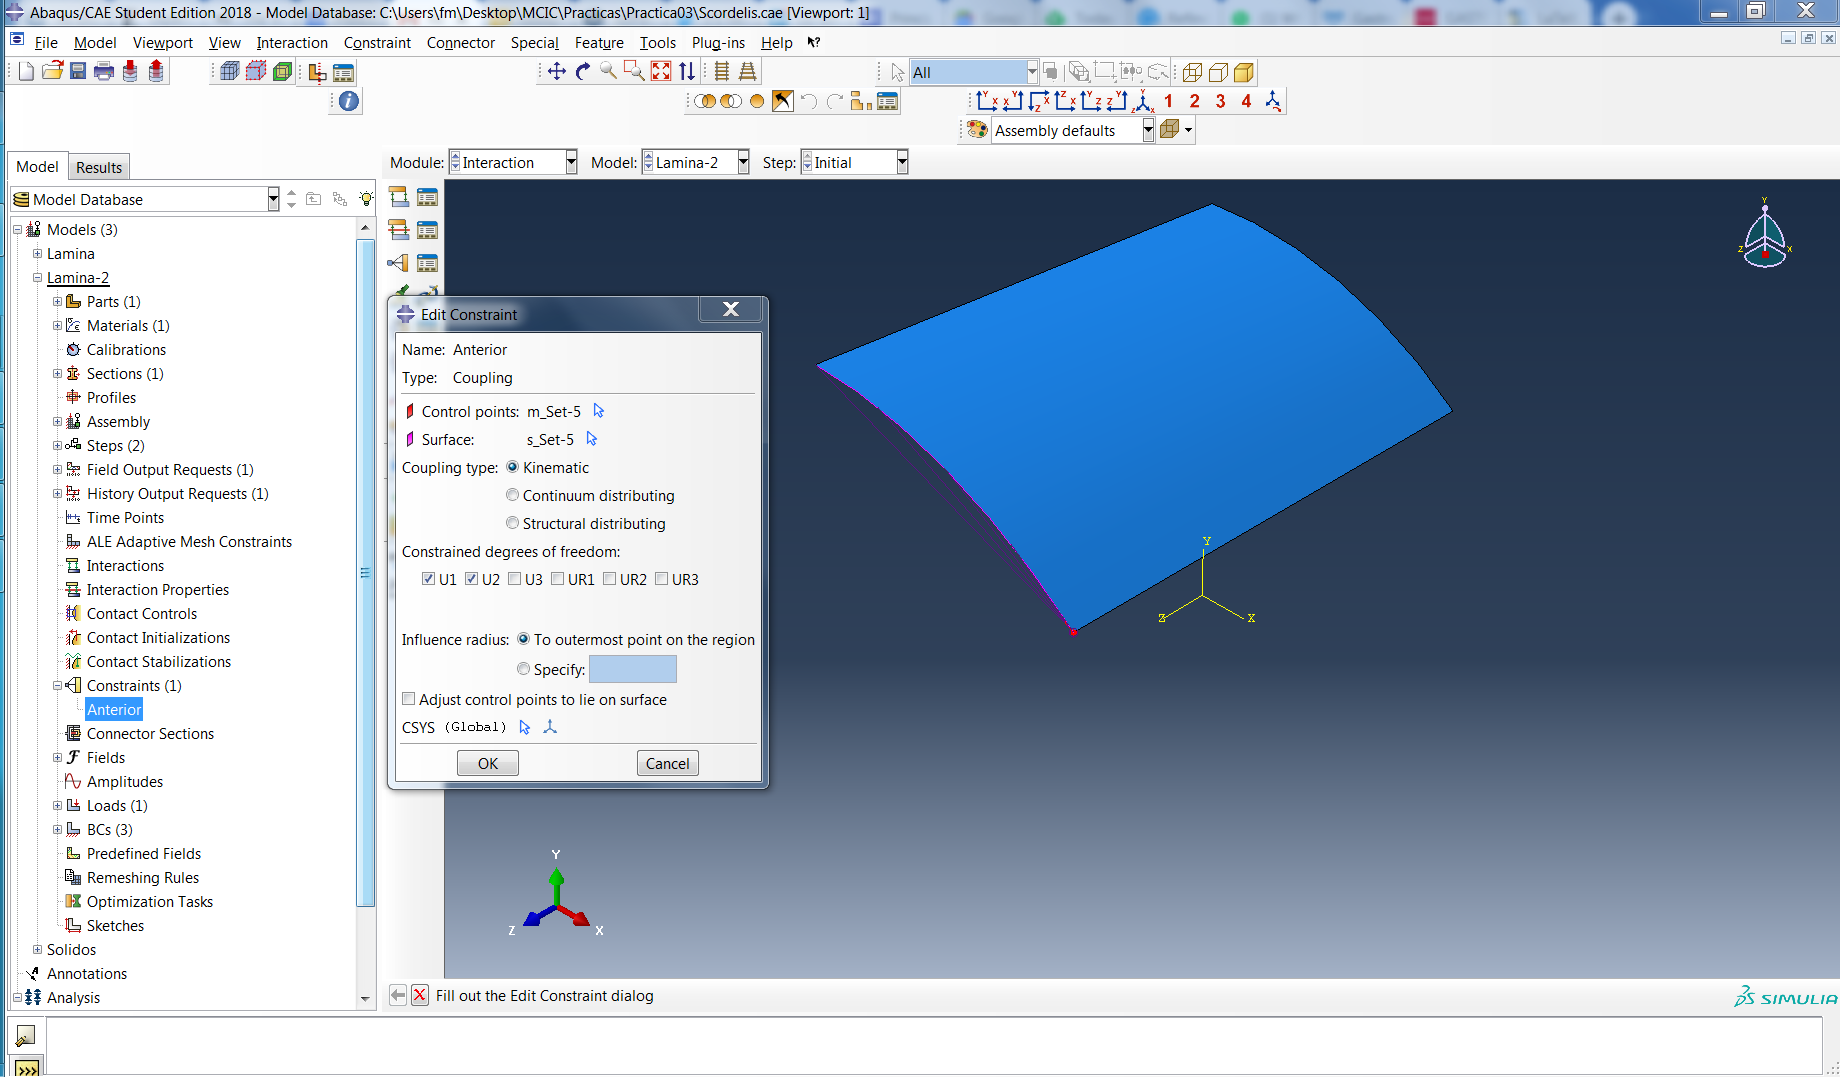
\includegraphics{Fig-7_Kinematic_constraint.png}

\centering{Figura 7: Asignaci�n{\it kinematic coupling}}
\vspace{3cm}

Se asigna la condici�n de contorno al nodo maestro:
\vspace{1cm}

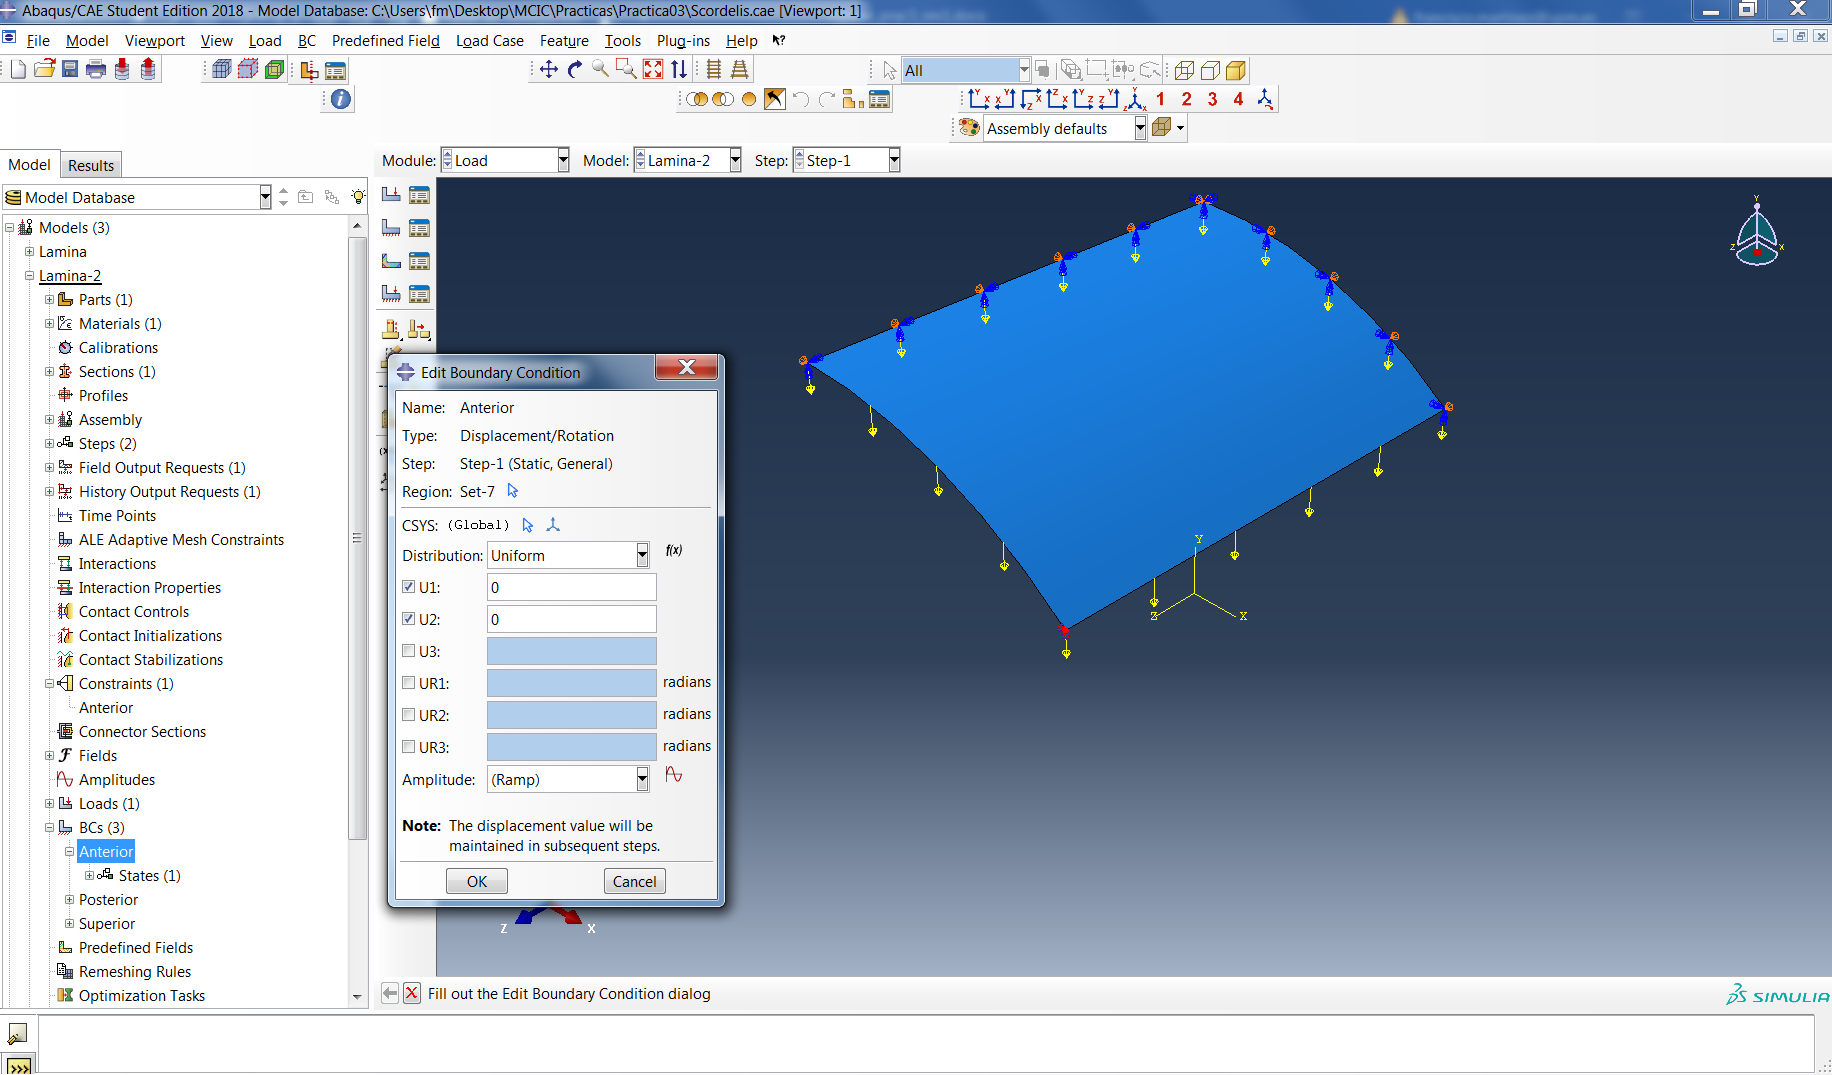
\includegraphics{Fig-8_BC_Nodo_Maestro.png}

\centering{Figura 8: Asignaci�n condici�n de contorno}
\vspace{3cm}

Si se hace as� el resultado es completamente exacto como se puede apreciar en la imagen siguiente.




\vspace{1cm}

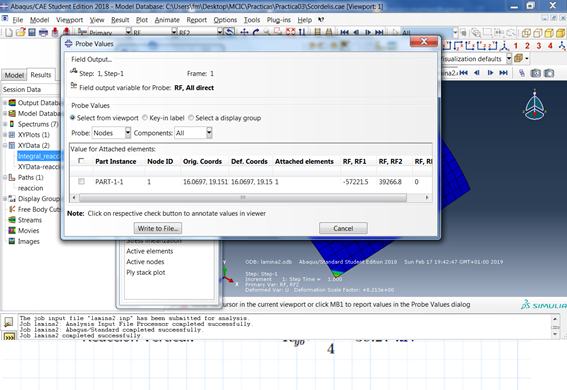
\includegraphics{Fig-9_Kinematic_Reacc_Vertical.png}

\centering{Figura 7: C�lculo reacci�n mediante {\it kinematic coupling}}
\vspace{3cm}


\end{document}
